\section{Reresultater}

Ud fra vores accepttest blev alle vores krav testet. Resultaterne giver et billede over hvilke funktioner som virkede optimalt, og hvilke der ikke gjorde. 

\begin{table}[h!]
	\centering
	\begin{tabular}{llllll}
		\multicolumn{6}{l}{\cellcolor[HTML]{187ABD}\textbf{Resultater for accepttest af Use Case 1: Mål og vis blodtryk og puls}} \\ \hline
		\textbf{Use Case 1: Mål og} & \multicolumn{1}{l|}{} &  & \multicolumn{1}{l|}{} & \textbf{Ext. 1: Digitalt filter} &  \\
		\textbf{vis blodtryk og puls} & \multicolumn{1}{l|}{} &  & \multicolumn{1}{l|}{} & \textbf{vælges fra} &  \\ \cline{1-2} \cline{5-6} 
		\textbf{Test} & \multicolumn{1}{l|}{\textbf{Resultat}} &  & \multicolumn{1}{l|}{} & \textbf{Test} & \textbf{Resultat} \\ \cline{1-2} \cline{5-6} 
		1.1 & \multicolumn{1}{l|}{OK} &  & \multicolumn{1}{l|}{} & 1.2.1 & OK \\ \cline{1-2} \cline{5-6} 
		1.2 & \multicolumn{1}{l|}{OK} &  & \multicolumn{1}{l|}{} &  &  \\ \cline{1-2} \cline{5-6} 
		1.3 & \multicolumn{1}{l|}{OK} &  & \multicolumn{1}{l|}{} &  &  \\ \cline{1-2} \cline{5-6} 
		1.4 & \multicolumn{1}{l|}{OK} &  & \multicolumn{1}{l|}{} &  & 
	\end{tabular}
\end{table}

\begin{table}[h!]
	\centering
	\begin{tabular}{llllll}
		\multicolumn{6}{l}{\cellcolor[HTML]{187ABD}\textbf{Resultater for accepttest af Use Case 2: Juster grænseværdier}} \\ \hline
		\textbf{Use Case 2: Juster} & \multicolumn{1}{l|}{} &  & \multicolumn{1}{l|}{} & \textbf{Ext. 2a: Systemet} &  \\
		\textbf{grænseværdier} & \multicolumn{1}{l|}{} &  & \multicolumn{1}{l|}{} & \textbf{afviser justering} &  \\ \cline{1-2} \cline{5-6} 
		\textbf{Test} & \multicolumn{1}{l|}{\textbf{Resultat}} &  & \multicolumn{1}{l|}{} & \textbf{Test} & \textbf{Resultat} \\ \cline{1-2} \cline{5-6} 
		2.1 & \multicolumn{1}{l|}{OK} &  & \multicolumn{1}{l|}{} & 2.1.1 & OK \\ \cline{1-2} \cline{5-6} 
		2.2 & \multicolumn{1}{l|}{OK} &  & \multicolumn{1}{l|}{} & 2.1.2 & FAIL \\ \cline{1-2} \cline{5-6} 
		2.3 & \multicolumn{1}{l|}{OK} &  & \multicolumn{1}{l|}{} & 2.1.3 & OK \\ \cline{1-2} \cline{5-6} 
		2.4 & \multicolumn{1}{l|}{OK} &  & \multicolumn{1}{l|}{} & 2.1.4 & Ikke testet
	\end{tabular}
\end{table}

\begin{table}[h!]
	\centering
	\begin{tabular}{llllll}
		\multicolumn{6}{l}{\cellcolor[HTML]{187ABD}\textbf{Resultater for accepttest af Use Case 3: Alarmering}} \\ \hline
		\textbf{Use Case 3:} & \multicolumn{1}{l|}{} &  & \multicolumn{1}{l|}{} & \textbf{Ext. 3a: Sundheds-} &  \\
		\textbf{Alarmering} & \multicolumn{1}{l|}{} &  & \multicolumn{1}{l|}{} & \textbf{fagligt personale} &  \\
		& \multicolumn{1}{l|}{} &  & \multicolumn{1}{l|}{} & \textbf{muter alarmen} &  \\ \cline{1-2} \cline{5-6} 
		\textbf{Test} & \multicolumn{1}{l|}{\textbf{Resultat}} &  & \multicolumn{1}{l|}{} & \textbf{Test} & \textbf{Resultat} \\ \cline{1-2} \cline{5-6} 
		(Hovedscenarie testet & \multicolumn{1}{l|}{} &  & \multicolumn{1}{l|}{} & 3.1.1 & OK \\ \cline{5-6} 
		gennem andre Use & \multicolumn{1}{l|}{} &  & \multicolumn{1}{l|}{} & 3.1.2 & OK \\ \cline{5-6} 
		Cases) & \multicolumn{1}{l|}{} &  & \multicolumn{1}{l|}{} & 3.1.3 & OK
	\end{tabular}
\end{table}

\begin{table}[h!]
	\centering
	\begin{tabular}{llllll}
		\multicolumn{6}{l}{\cellcolor[HTML]{187ABD}\textbf{Resultater for accepttest af Use Case 4: Gem data}} \\ \hline
		\textbf{Use Case 4: Gem} & \multicolumn{1}{l|}{} &  & \multicolumn{1}{l|}{} & \textbf{Ext. 4a: Data ikke} &  \\
		\textbf{data} & \multicolumn{1}{l|}{} &  & \multicolumn{1}{l|}{} & \textbf{gemt} &  \\ \cline{1-2} \cline{5-6} 
		\textbf{Test} & \multicolumn{1}{l|}{\textbf{Resultat}} &  & \multicolumn{1}{l|}{} & \textbf{Test} & \textbf{Resultat} \\ \cline{1-2} \cline{5-6} 
		4.1 & \multicolumn{1}{l|}{OK} &  & \multicolumn{1}{l|}{} & 4.1.1 & FAIL \\ \cline{1-2} \cline{5-6} 
		4.2 & \multicolumn{1}{l|}{FAIL} &  & \multicolumn{1}{l|}{} & 4.1.2 & FAIL \\ \cline{1-2} \cline{5-6} 
		4.3 & \multicolumn{1}{l|}{FAIL} &  & \multicolumn{1}{l|}{} &  &  \\ \cline{1-2} \cline{5-6} 
		4.4 & \multicolumn{1}{l|}{FAIL} &  & \multicolumn{1}{l|}{} &  & 
	\end{tabular}
\end{table}

\clearpage

\begin{table}[h!]
	\centering
	\begin{tabular}{ll}
		\multicolumn{2}{l}{\cellcolor[HTML]{187ABD}\textbf{Resultater for accepttest af Use Case 4: Kalibrering}} \\ \hline
		\multicolumn{1}{l|}{\textbf{Use Case 4: Kalibrering}} &  \\ \hline
		\multicolumn{1}{l|}{\textbf{Test}} & \textbf{Resultat} \\ \hline
		\multicolumn{1}{l|}{5.1} & OK \\ \hline
		\multicolumn{1}{l|}{5.2} & OK \\ \hline
		\multicolumn{1}{l|}{5.3} & FAIL \\ \hline
		\multicolumn{1}{l|}{5.4} & FAIL
	\end{tabular}
\end{table}

Ud over de ovenstående tests af funktionelle krav er der også blevet lavet acceptests af de ikke-funktionelle krav. Resultaterne på testen ses her: 

\begin{table}[h!]
	\centering
	\begin{tabular}{lll}
		\multicolumn{3}{l}{\cellcolor[HTML]{187ABD}\textbf{Resultater for ikke-funktionelle krav}} \\ \hline
		\multicolumn{1}{l|}{\textbf{Krav nr.}} & \multicolumn{1}{l|}{\textbf{Krav}} & \textbf{Vurdering} \\
		\multicolumn{1}{l|}{} & \multicolumn{1}{l|}{} & \textbf{(OK/FAIL)} \\ \hline
		\multicolumn{1}{l|}{1} & \multicolumn{1}{l|}{Den skærm der benyttes af operatøren} & OK \\
		\multicolumn{1}{l|}{} & \multicolumn{1}{l|}{er den skærm, hvor man kan interagere} &  \\
		\multicolumn{1}{l|}{} & \multicolumn{1}{l|}{med systemet} &  \\ \hline
		\multicolumn{1}{l|}{2} & \multicolumn{1}{l|}{Den skærm, der benyttes af observatøren} & Ikke testet \\
		\multicolumn{1}{l|}{} & \multicolumn{1}{l|}{er den skærm, hvor man observerer grafen} &  \\
		\multicolumn{1}{l|}{} & \multicolumn{1}{l|}{samt værdier for systolisk-, diastolisk-, middel-} &  \\
		\multicolumn{1}{l|}{} & \multicolumn{1}{l|}{blodtryk og puls.} &  \\ \hline
		\multicolumn{1}{l|}{3} & \multicolumn{1}{l|}{Systemets GUI skal indeholde elementerne} & OK \\
		\multicolumn{1}{l|}{} & \multicolumn{1}{l|}{beskrevet under systembeskrivelsen i dokumentet} &  \\
		\multicolumn{1}{l|}{} & \multicolumn{1}{l|}{"Kravspecifikation" som findes i bilaget} &  \\ \hline
		\multicolumn{1}{l|}{4} & \multicolumn{1}{l|}{Systemets GUI skal kunne vise en graf inden for} & OK \\
		\multicolumn{1}{l|}{} & \multicolumn{1}{l|}{5 sekunder} &  \\ \hline
		\multicolumn{1}{l|}{5} & \multicolumn{1}{l|}{Systemet skal kunne stoppe målingen inden for} & OK \\
		\multicolumn{1}{l|}{} & \multicolumn{1}{l|}{5 sekunder} &  \\ \hline
		\multicolumn{1}{l|}{6} & \multicolumn{1}{l|}{Grafen samt de viste værdier skal kunne læses på} & OK \\
		\multicolumn{1}{l|}{} & \multicolumn{1}{l|}{op til 0,5 meters afstand. Farverne skal kunne skelnes} &  \\
		\multicolumn{1}{l|}{} & \multicolumn{1}{l|}{af personer med farveblindhed} & 
	\end{tabular}
\end{table}

Gruppen fik lov til at komme ud på Skejby sygehus og afprøve blodtryksmåleren på en gris. Forsøget gik ikke helt som forventet. Vi havde forventet nogle større udsving og har efterfølgende fundet ud af, at filteret havde to forkerte modstande på printpladen. Dette var skyld i en for hård filtrering af signalet og er efterfølgende blevet ændret.

\vspace{0.5 cm}
\begin{figure}[h!]
	\centering
	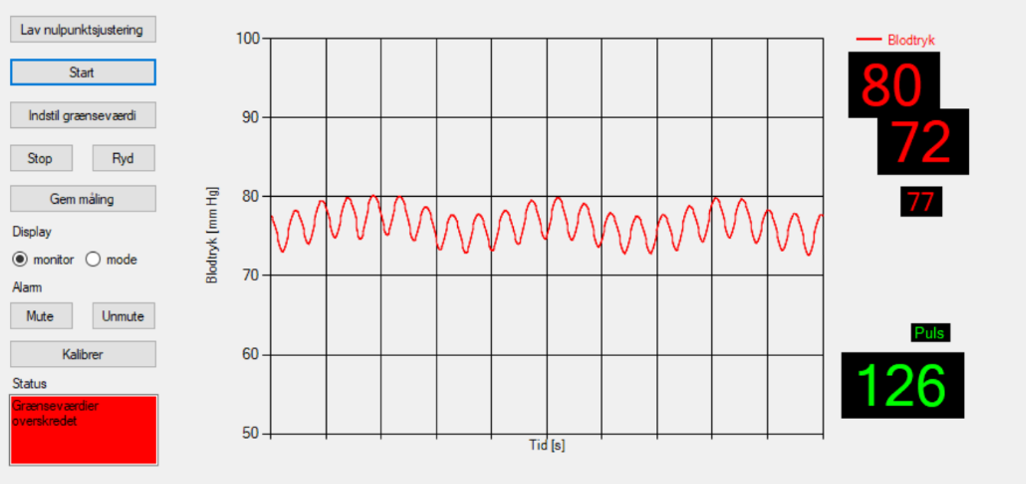
\includegraphics[width=0.7\linewidth]{Resultater/Resultater/gris}
	\label{fig:gris}
	\caption{Målt blodtryk på gris}
\end{figure}

\section{Diskussion af resultater}

Accepttesten gik udmærket, og vi fik valideret vores krav. Accepttesen bestod af 5 Use Cases, hvor hver Use Case indeholdt flere krav, der skulle testes. De fleste af kravene blev imødekommet, dog var der også flere som ikke gjorde. Kravene der ikke blev imødekommet skyldtes prioritering af forskellige arbejdsopgaver, hvor det var blevet nødvendigt at lægge arbejdsindsatsen ind på, at få alle ”Must have” kravene opfyldt, som det første.
Den første Use Case med ”Mål og vis blodtryk og puls” gik efter planen, og opfyldte alle de stillede krav. I denne Use Case var det de mest grundlæggende dele af vores system, som blev testet og var derfor prioriteret højt ift. at skulle bestå alle testene. Det lykkedes os at få foretaget en nulpunktsjustering samt at få vist blodtryk og puls på en graf via brugergrænsefladen, hvor grafen både kunne vises med digitalt filter og uden. 

Use Case 2 ”Justering af grænseværdier” gik som vi havde forventet. Det lykkedes os at kunne justere forskellige grænseværdier, hvor der kom en fejlmeddelelse, hvis grænserne virkede usandsynlige høje/lave.  En overskridning af grænseværdierne viste sig også fint i ”statusboksen”, som blinkede rødt og gav en alarmeringsbesked. Det lykkedes os dog ikke at få udført en ændring af grænseværdierne mens vi fik et signal ind, da testen ikke kunne udføres med signalet fra væskesøjlen. Væskesøjlen giver en puls på 0, og vil derfor gøre det umuligt for os at teste på, da der ikke kan justeres på pulsen. I stedet skulle der have været brugt en analog discovery til at sende et signal ind.

Use Case 3 ” Alarmering” blev testet parallelt med andre use cases idet de aktiverede alarmerne i forskellige sammenhænge. Vi valgte derfor ikke at lave nogle specifikke test af alarmen, udover hvor alarmen mutes. Når alarmen var i gang auditivt spillede tonerne c e g – g C, hvilket var det vi havde forventet. Samtidigt blinkede ”statusboksen” med en hertz på 2, og en duty cycle på 50%. 

Det lykkedes os desværre ikke at gemme vores data, som planlagt i Use Case 4 ”Gem data”. Efter at have gået vores kode for ”gem data” grundigt igennem står det nu klart for os, hvorfor data’en ikke bliver gemt. I koden bliver der oprettet nye instanser af hver klasse, hver gang der skal gemmes noget data. Dette medfører at data’en fra den klasse, som der gerne skulle gemmes fra ikke bliver overført til klassen, hvor vi gerne vil gemme det. Resultatet af det er at vi ikke får gemt noget data.
Udover at have oprettet flere instanser af klasserne opstod der også problemer under serialisering af den gemte data. 

Under testning af kalibreringen fandt vi ud af at vores system kalibrer korrekt, dog blev den lineære regression ikke udført korrekt.

Accepttesten forløb godt trods de fejl, som er opstået. Systemet opfyldte alle vores ikke-funktionelle krav, og de fleste funktionelle krav til systemet blev imødekommet. Accepttesten giver et billede af hvad vi har prioriteret højtest af krav.
